\begin{figure}
	\centering
	\begin{subfigure}{0.48\columnwidth}
		\centering
		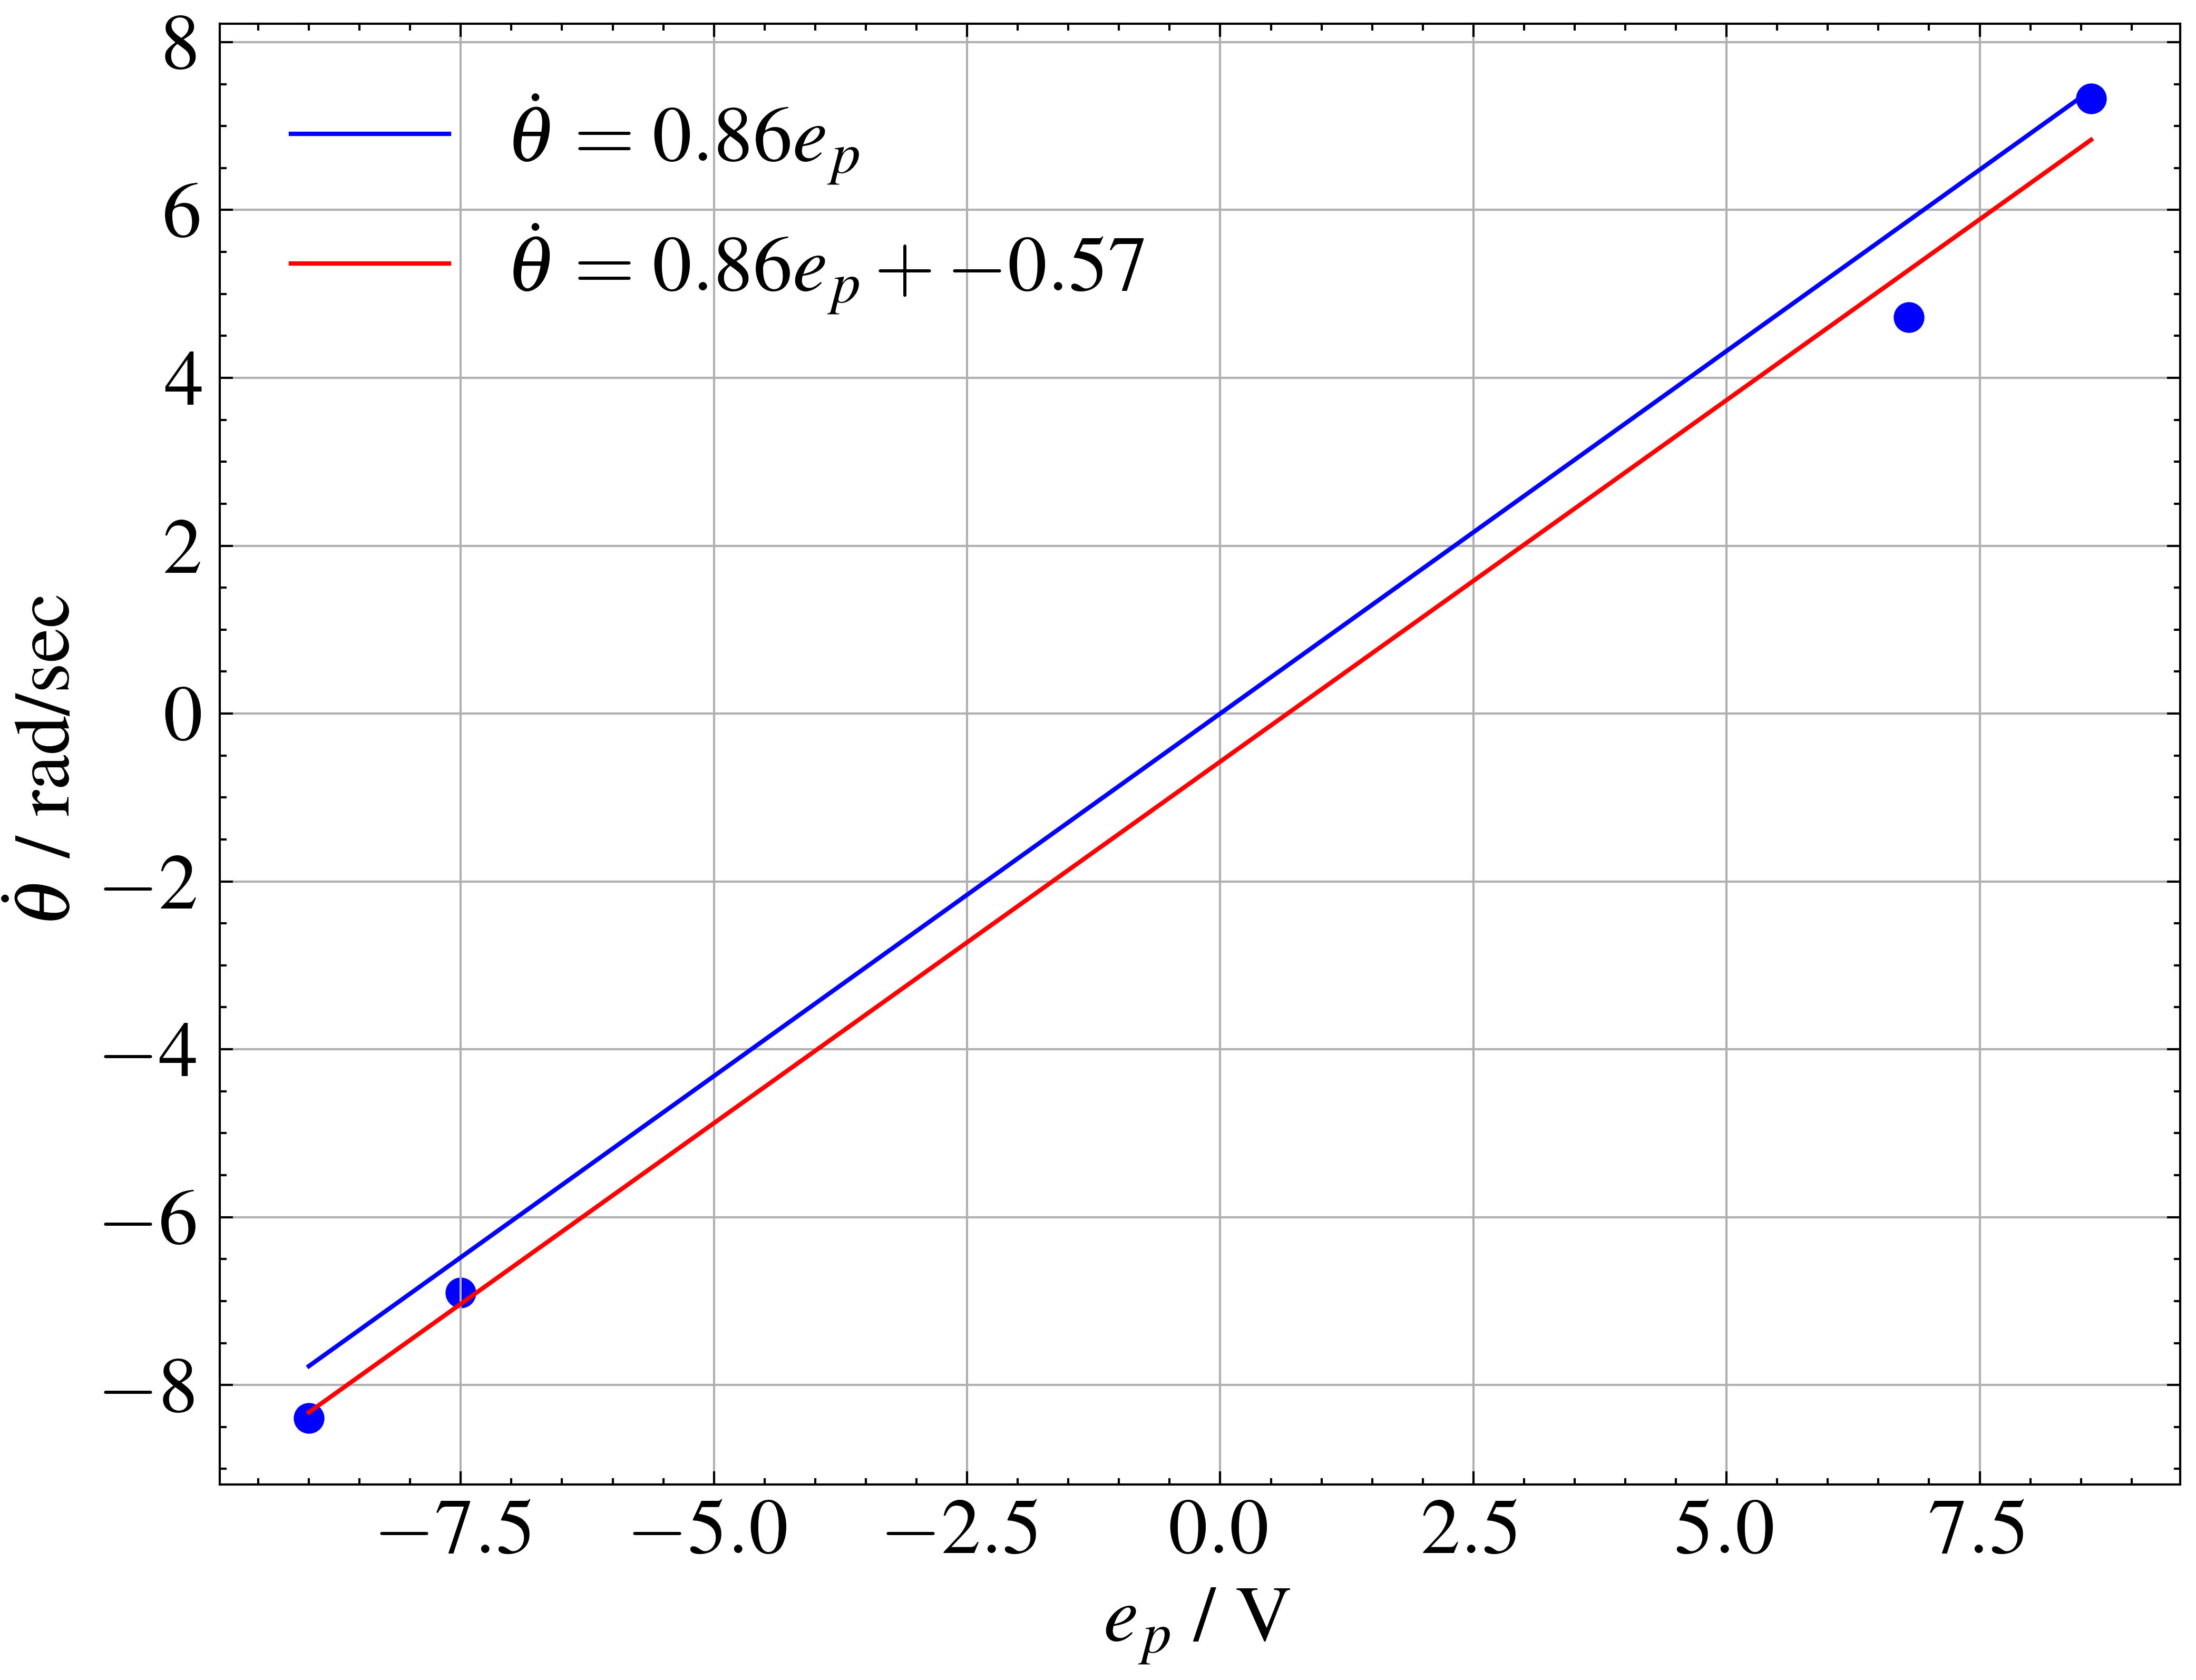
\includegraphics[width=0.8\linewidth]{src/figures/theta_dot-e_p-relation/theta_dot-e_p-relation-P60.png}
		\subcaption{$P=60$}
	\end{subfigure}
	\begin{subfigure}{0.48\columnwidth}
		\centering
		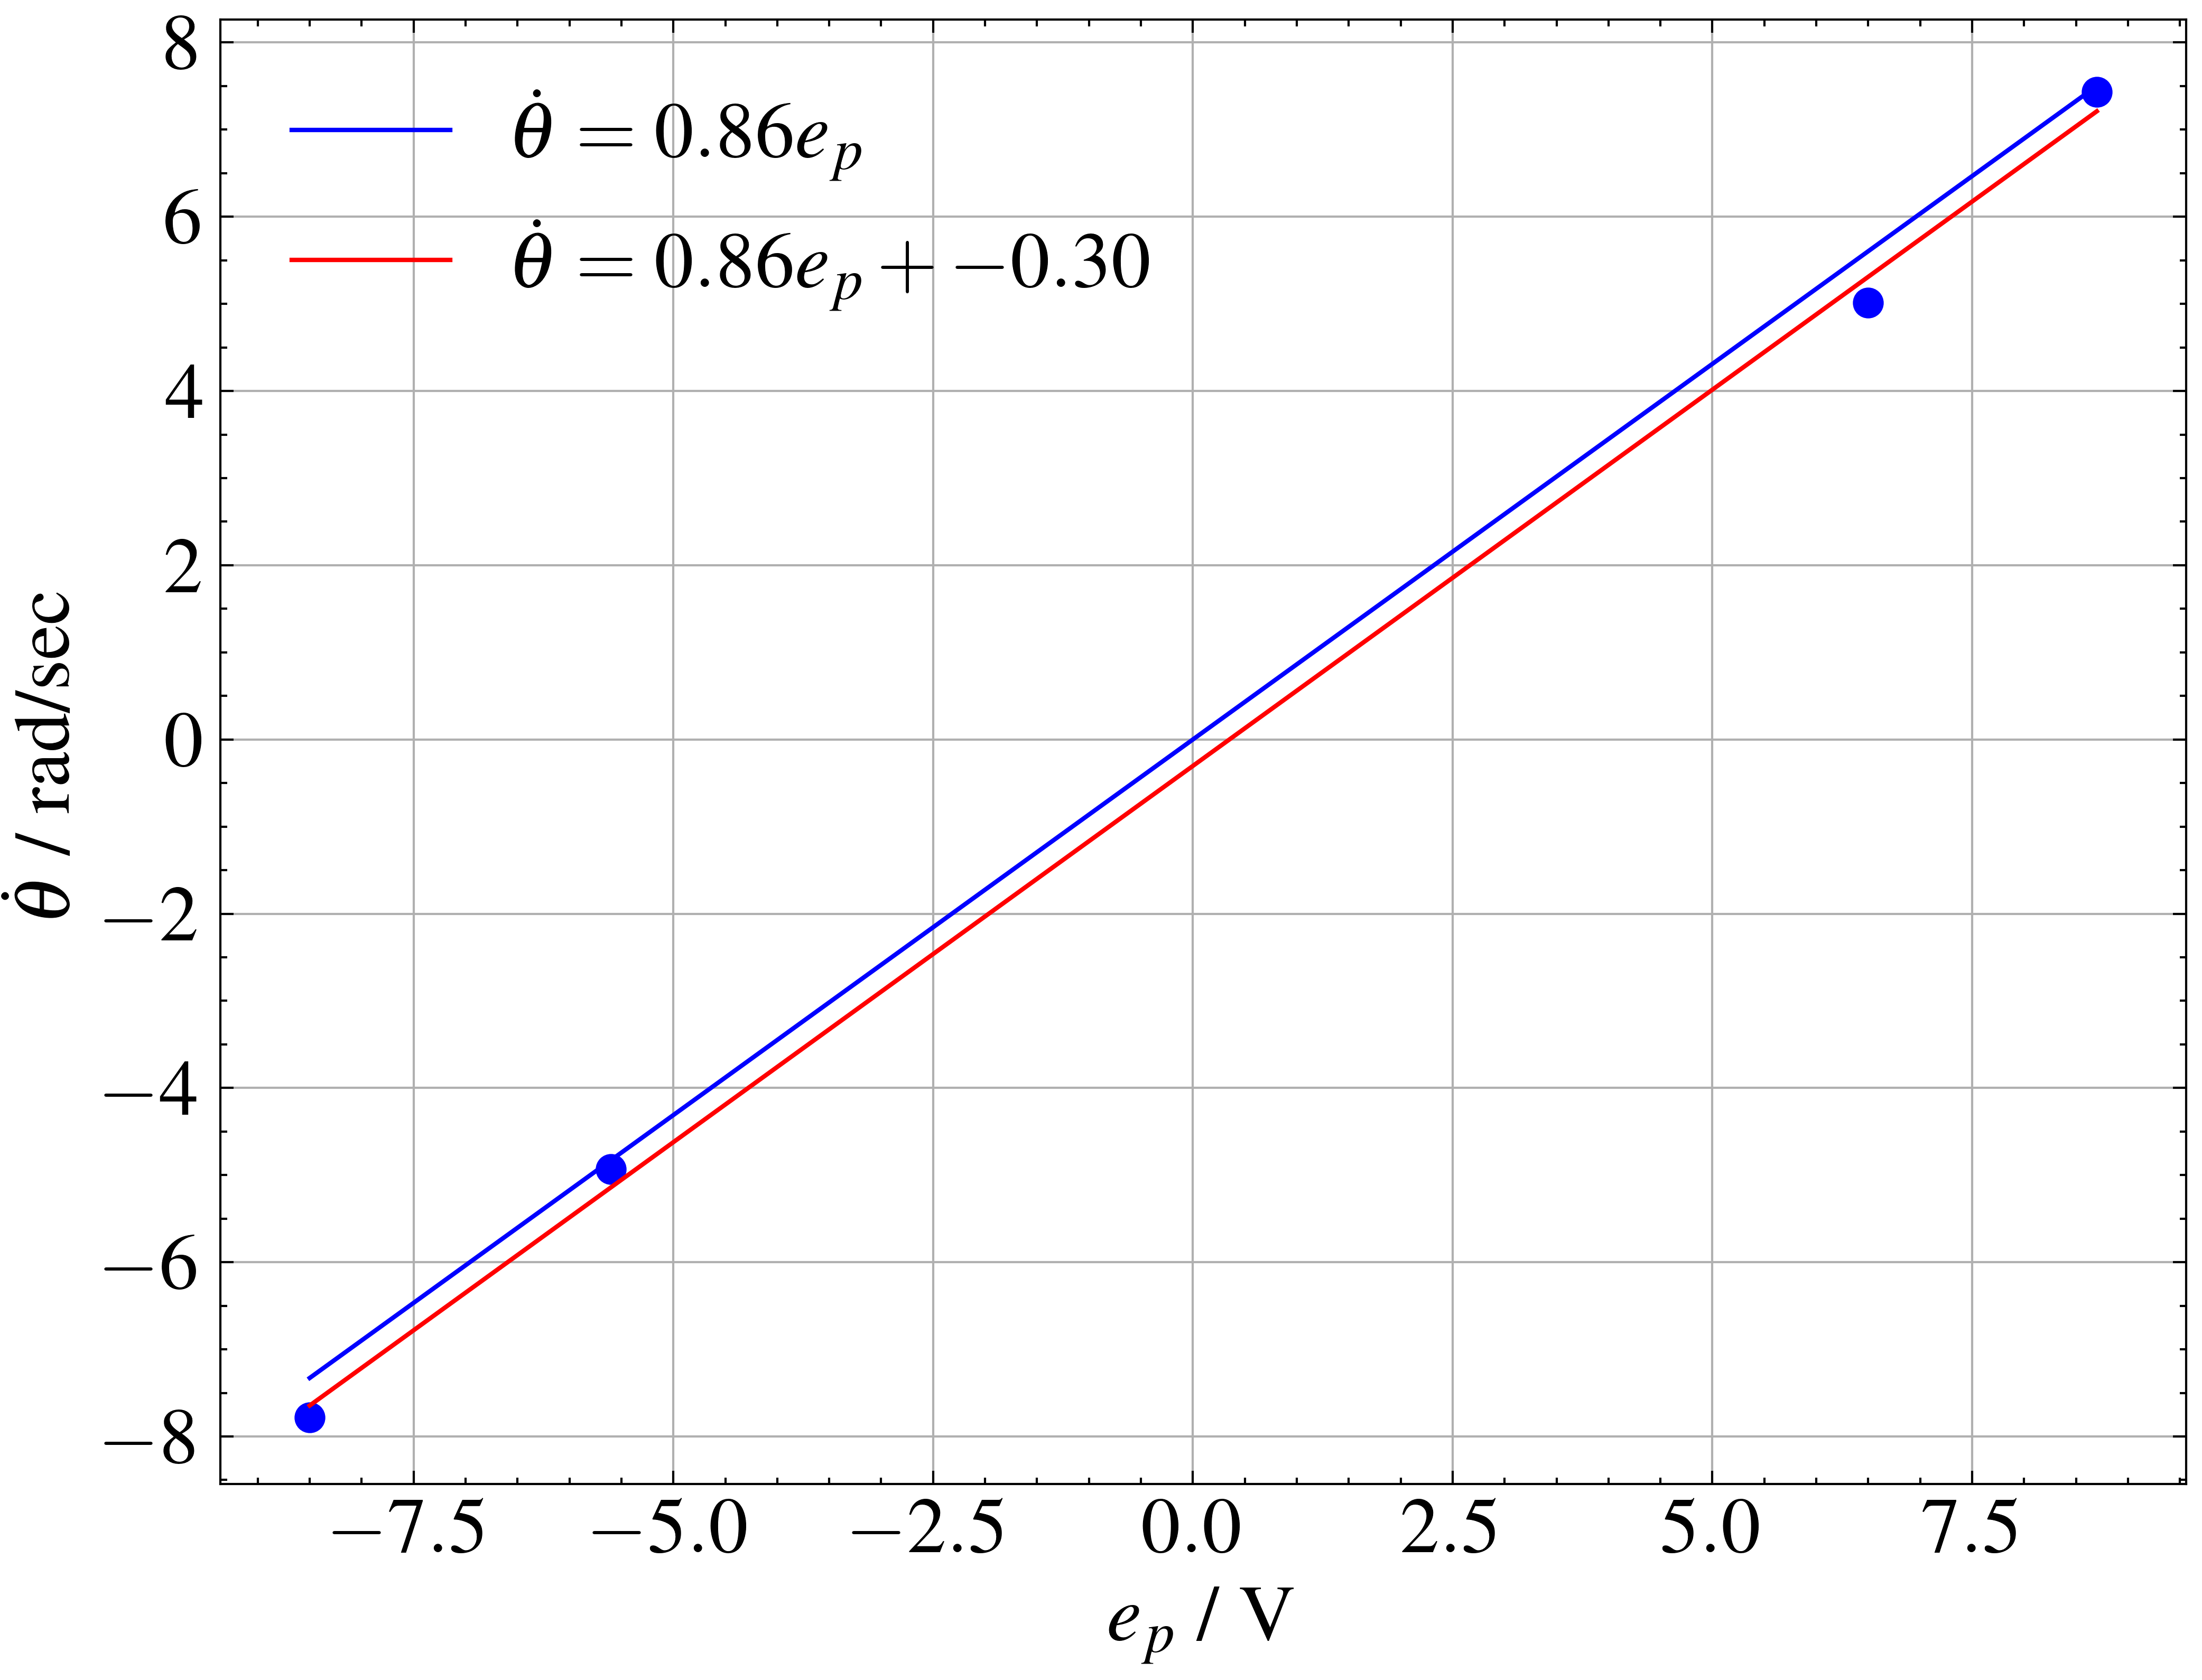
\includegraphics[width=0.8\linewidth]{src/figures/theta_dot-e_p-relation/theta_dot-e_p-relation-P80.png}
		\subcaption{$P=80$}
	\end{subfigure}
	\begin{subfigure}{0.48\columnwidth}
		\centering
		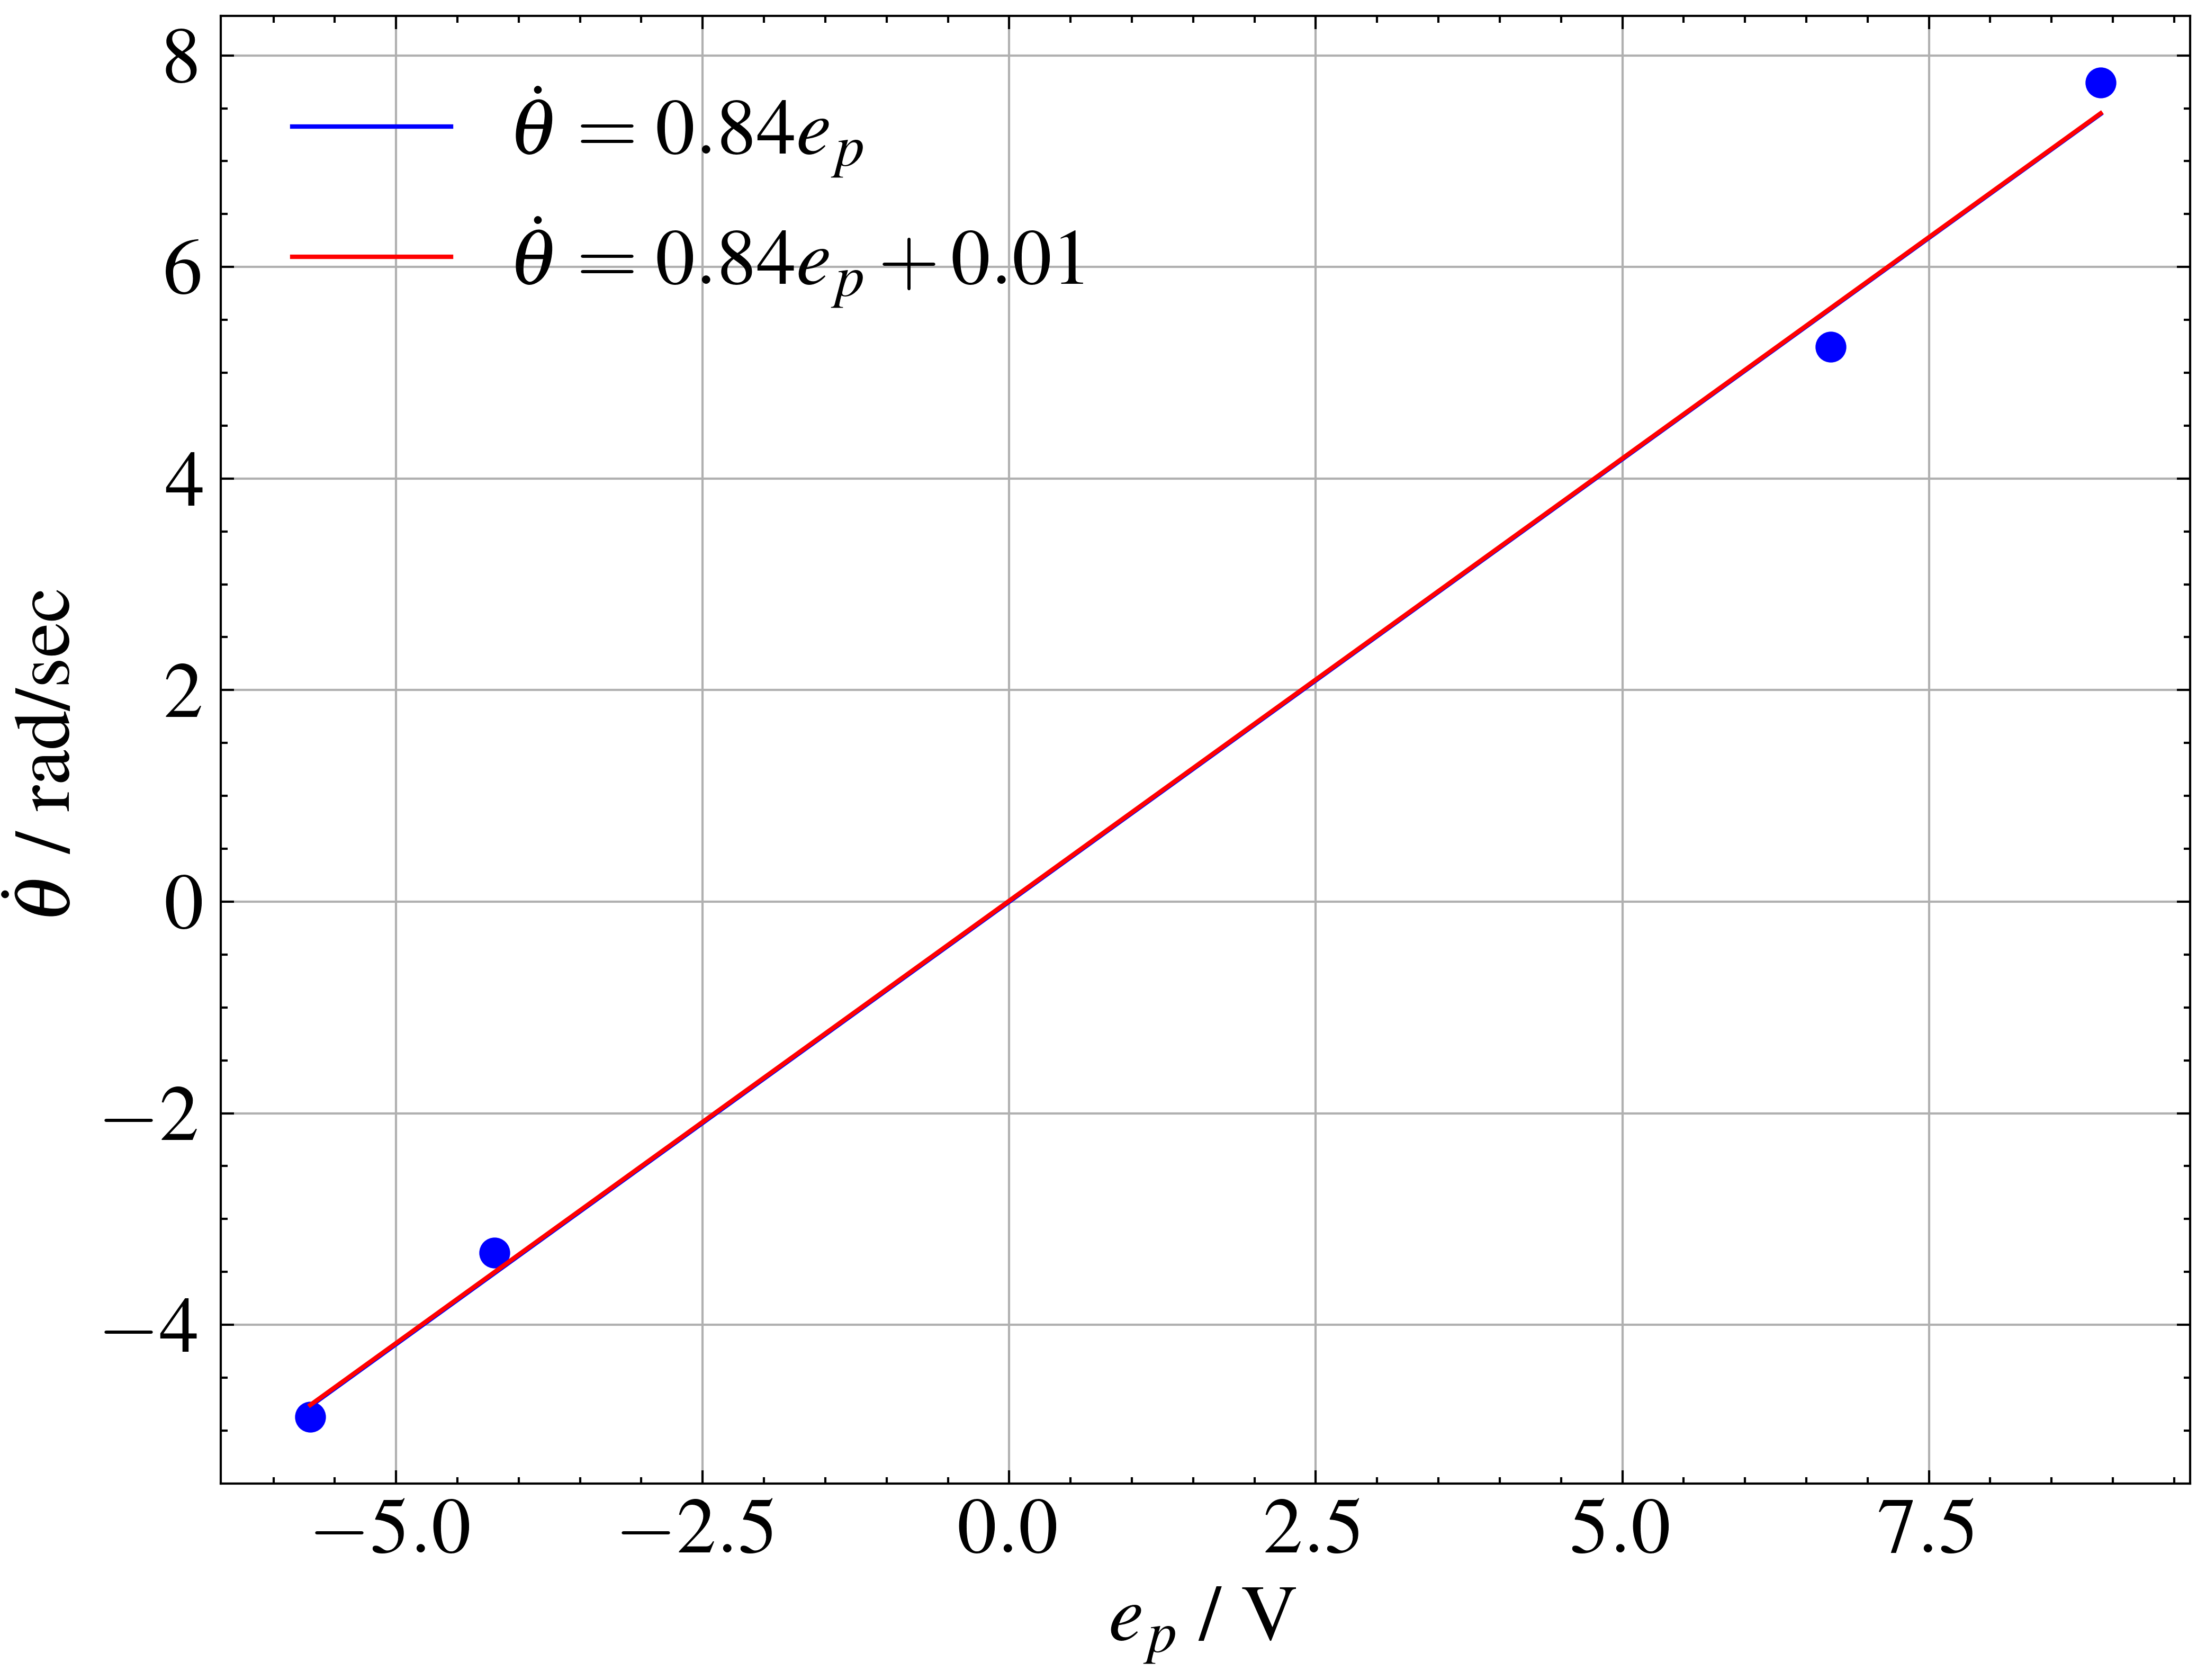
\includegraphics[width=0.8\linewidth]{src/figures/theta_dot-e_p-relation/theta_dot-e_p-relation-P100.png}
		\subcaption{$P=100$}
	\end{subfigure}
	\caption{$P$に対する$e_p$と$\dot{\theta_2}$の関係}\label{fig:theta_dot-e_p-relation}
\end{figure}
